%!TEX root = ../thesis.tex

\chapter{Perturbation series}

\usetikzlibrary{decorations.markings}

\pgfdeclaredecoration{waves}{start}{
    \state{start}[width=0pt, next state=positive, persistent precomputation={
        \pgfmathsetlengthmacro\pgfdecorationsegmentlength{
            \pgfdecoratedinputsegmentlength / int(2
                * \pgfdecoratedinputsegmentlength
                / \pgfdecorationsegmentlength
                )
            }
        }] \relax
    \state{positive}[width=\pgfdecorationsegmentlength, next state=negative]{
        \pgfpathsine{\pgfpoint
            {\pgfdecorationsegmentlength/2}
            {\pgfdecorationsegmentamplitude/2}
            }
        \pgfpathcosine{\pgfpoint
            {\pgfdecorationsegmentlength/2}
            {\pgfdecorationsegmentamplitude/-2}
            }
        }
    \state{negative}[width=\pgfdecorationsegmentlength, next state=positive]{
        \pgfpathsine{\pgfpoint
            {\pgfdecorationsegmentlength/2}
            {\pgfdecorationsegmentamplitude/-2}
            }
        \pgfpathcosine{\pgfpoint
            {\pgfdecorationsegmentlength/2}
            {\pgfdecorationsegmentamplitude/2}
            }
        }
    \state{final}{\pgfpathmoveto\pgfpointdecoratedpathlast}
    }

\tikzset{electron/.style={
    thick,
    decoration={markings, mark=at position 0.5 with {\arrow>}},
    postaction={decorate},
    }}

\tikzset{phonon/.style={
    thick,
    decoration={waves, amplitude=2mm/3, segment length=2mm},
    decorate,
    }}

\begin{figure}
    \small
    \medmuskip=0mu
    \begin{subfigure}[b]{\linewidth/3}
        \centering
        \tikzsetnextfilename{hartree}
        % !TEX root = ../thesis.tex
%
\tikzsetnextfilename{hartree}
%
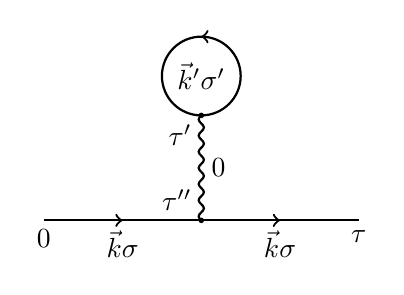
\begin{tikzpicture}
    \coordinate (i) at (0, 0);
    \coordinate (2) at (2, 0);
    \coordinate (1) at (2, 4/3);
    \coordinate (o) at (4, 0);

    \draw [phonon] (2) -- node [right] {$0$} (1);

    \draw [electron] (i) -- node [below] {$\vec k \sigma$} (2);
    \draw [electron] (2) -- node [below] {$\vec k \sigma$} (o);

    \draw [electron] (1) arc (-90:270:5mm)
        node [yshift=5mm] {$\vec k' \sigma'$};

    \foreach \point in {1, 2} \fill (\point) circle (1pt);

    \node [below] at (i) {$0$};
    \node [above left] at (2) {$\tau''$};
    \node [below left] at (1) {$\tau'$};
    \node [below] at (o) {$\tau$};

    \useasboundingbox ([yshift=1mm] current bounding box.north east);
\end{tikzpicture}%

        \caption{Hartree}
    \end{subfigure}%
    \begin{subfigure}[b]{\linewidth/3}
        \centering
        \tikzsetnextfilename{fock}
        % !TEX root = ../thesis.tex
%
\tikzsetnextfilename{fock}
%
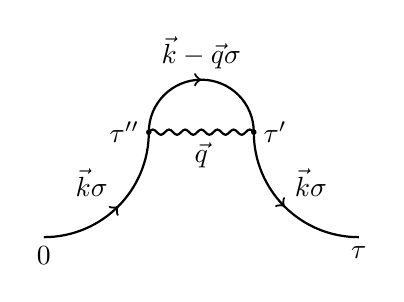
\begin{tikzpicture}[bend angle=45]
    \coordinate (i) at (0, 0);
    \coordinate (2) at (4/3, 4/3);
    \coordinate (t) at (6/3, 6/3);
    \coordinate (1) at (8/3, 4/3);
    \coordinate (o) at (4, 0);

    \draw [phonon] (2) -- node [below] {$\vec q$} (1);

    \draw [electron] (i) to [bend right]
        node [above left] {$\vec k \sigma$} (2);
    \draw [electron] (2) to [bend left] (t)
        node [above] {$\vec k - \vec q \sigma$} to [bend left] (1);
    \draw [electron] (1) to [bend right]
        node [above right] {$\vec k \sigma$} (o);

    \foreach \point in {1, 2} \fill (\point) circle (1pt);

    \node [below] at (i) {$0$};
    \node [left] at (2) {$\tau''$};
    \node [right] at (1) {$\tau'$};
    \node [below] at (o) {$\tau$};
\end{tikzpicture}%

        \caption{Fock}
    \end{subfigure}%
    \begin{subfigure}[b]{\linewidth/3}
        \centering
        \tikzsetnextfilename{fock-anomalous}
        \input{tikzin/fock-anomalous.tex}
        \caption{Fock, anomalous}
    \end{subfigure}\\[1cm]
    \begin{subfigure}[b]{\linewidth/3}
        \centering
        \tikzsetnextfilename{glasses}
        % !TEX root = ../thesis.tex
%
\tikzsetnextfilename{glasses}
%
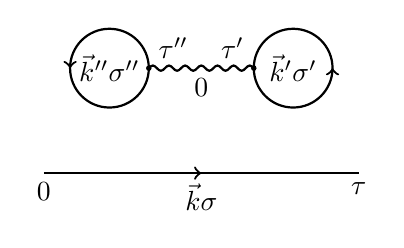
\begin{tikzpicture}
    \coordinate (i) at (0, 0);
    \coordinate (2) at (4/3, 4/3);
    \coordinate (1) at (8/3, 4/3);
    \coordinate (o) at (4, 0);

    \draw [phonon] (2) -- node [below] {$0$} (1);

    \draw [electron] (i) -- node [below] {$\vec k \sigma$} (o);

    \draw [electron] (2) arc (0:360:5mm)
        node [xshift=-5mm] {$\vec k'' \sigma''$};
    \draw [electron] (1) arc (180:540:0.5)
        node [xshift=5mm] {$\vec k' \sigma'$};

    \foreach \point in {1, 2} \fill (\point) circle (1pt);

    \node [below] at (i) {$0$};
    \node [above right] at (2) {$\tau''$};
    \node [above left] at (1) {$\tau'$};
    \node [below] at (o) {$\tau$};
\end{tikzpicture}%

        \caption{``Glasses''}
    \end{subfigure}%
    \begin{subfigure}[b]{\linewidth/3}
        \centering
        \tikzsetnextfilename{porthole}
        \input{tikzin/porthole.tex}
        \caption{``Porthole''}
    \end{subfigure}%
    \begin{subfigure}[b]{\linewidth/3}
        \centering
        \tikzsetnextfilename{porthole-anomalous}
        %!TEX root = ../thesis.tex
%
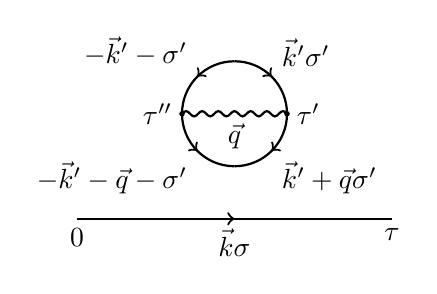
\begin{tikzpicture}[bend angle=45]
    \coordinate (i) at (0, 0);
    \coordinate (2) at (4/3, 4/3);
    \coordinate (t) at (6/3, 6/3);
    \coordinate (b) at (6/3, 2/3);
    \coordinate (1) at (8/3, 4/3);
    \coordinate (o) at (4, 0);
    %
    \draw [electron] (i) -- node [below] {$\vec k \sigma$} (o);
    %
    \draw [phonon] (2) -- node [below] {$\vec q$} (1);
    %
    \draw [electron] (t) to [bend left]
        node [above right] {$\vec k' \sigma'$} (1);
    \draw [electron] (t) to [bend right]
        node [above left] {$-\vec k' -\sigma'$} (2);
    %
    \draw [electron] (1) to [bend left]
        node [below right] {$\vec k' + \vec q \sigma'$} (b);
    \draw [electron] (2) to [bend right]
        node [below left] {$-\vec k' -\vec q -\sigma'$} (b);
    %
    \foreach \point in {1, 2} \fill (\point) circle (1pt);
    %
    \node [below] at (i) {$0$};
    \node [left] at (2) {$\tau''$};
    \node [right] at (1) {$\tau'$};
    \node [below] at (o) {$\tau$};
\end{tikzpicture}%

        \caption{``Porthole'', anomalous}
    \end{subfigure}
    \caption{2nd order \name{Feynman} graphs}
\end{figure}
